\section{Extensibility}
\label{design:extensibility}

In \autoref{design:communication} we mentioned a secondary communication mechanism that would be best implemented in form of an extension to the bootware.
The requirements for the bootware also state that support for different cloud environments and provisioning engines should be achieved through means of software engineering.
These requirements are intentionally vague to allow for the selection of a fitting extension mechanism during the design process.
In this section we will take a look at different extension mechanisms for Java and pick the one that suits our needs best.

\subsection{Extension Mechanisms}

The simplest way to fulfill the extensibility requirement would be to create a set of interface and abstract classes to define the interfaces and basic functionality that are necessary to work with different cloud environments and provisioning engines.
These interfaces and abstract classes would then be implemented separately to support different scenarios and would be compiled, together with the rest of the application, into one executable.
At runtime, a suitable implementation would be selected and used to execute the specific functionality required at this time.

This extension mechanism is simple, but restricted by its static nature.
The entire executable has to be recompiled if any implementations are changed or added.
This may not be a problem if the set of possible extensions that have to be supported is limited and known at the time of implementation or if it changes rarely.
If the set of necessary extensions is unknown or changing from time to time, implementing new or changing existing extensions can get cumbersome, since a new version of the whole software has to be released each time.
It would be far better if extensions could be implemented separately from the core bootware component and added and removed at will.

A more flexible architecture is needed, for example a plugin architecture.
Interfaces for the extension points still exist but the extension are no longer part of the main bootware component.
They are compiled separately into plugins that can be loaded into the main bootware component on the fly.
There are several possibilities to realize such an architecture.

It is certainly possible to implement a plugin framework from scratch.
An advantage of this approach would be that the design of the plugin architecture could be tailored to our use case and would be as simple or complex as needed.
But there are also several disadvantages.
For one, we would reinvent the wheel, since multiple such frameworks already exist.
It would also shift resources away from the actual goal of this thesis, which is designing the bootware component.
Furthermore it would require a deep understanding of the language used for the implementation (in this case Java), which is not necessarily given.
Therefore it seems more reasonable to use one of the already existing plugin frameworks.
Which one exactly will be determined later in \autoref{implementation:selecting:pluginframeworks}.

\subsection{Plugin Repository}
\label{design:pluginrepository}

Now that we have introduced plugins we face new problems.
\autoref{image:plugins} shows the current architecture, where both bootware components use their own plugins.
If a plugin is added or updated, the user has to manually copy this plugin to the right folder of one or both of the bootware components.
Furthermore, if both components use the same plugins, which they will (for example plugins for different cloud providers), we will have duplicate plugins scattered around.
This is inefficient, probably annoying for the user and can possibly cause errors if plugins get out of sync.

\begin{figure}[!htbp]
	\centering
	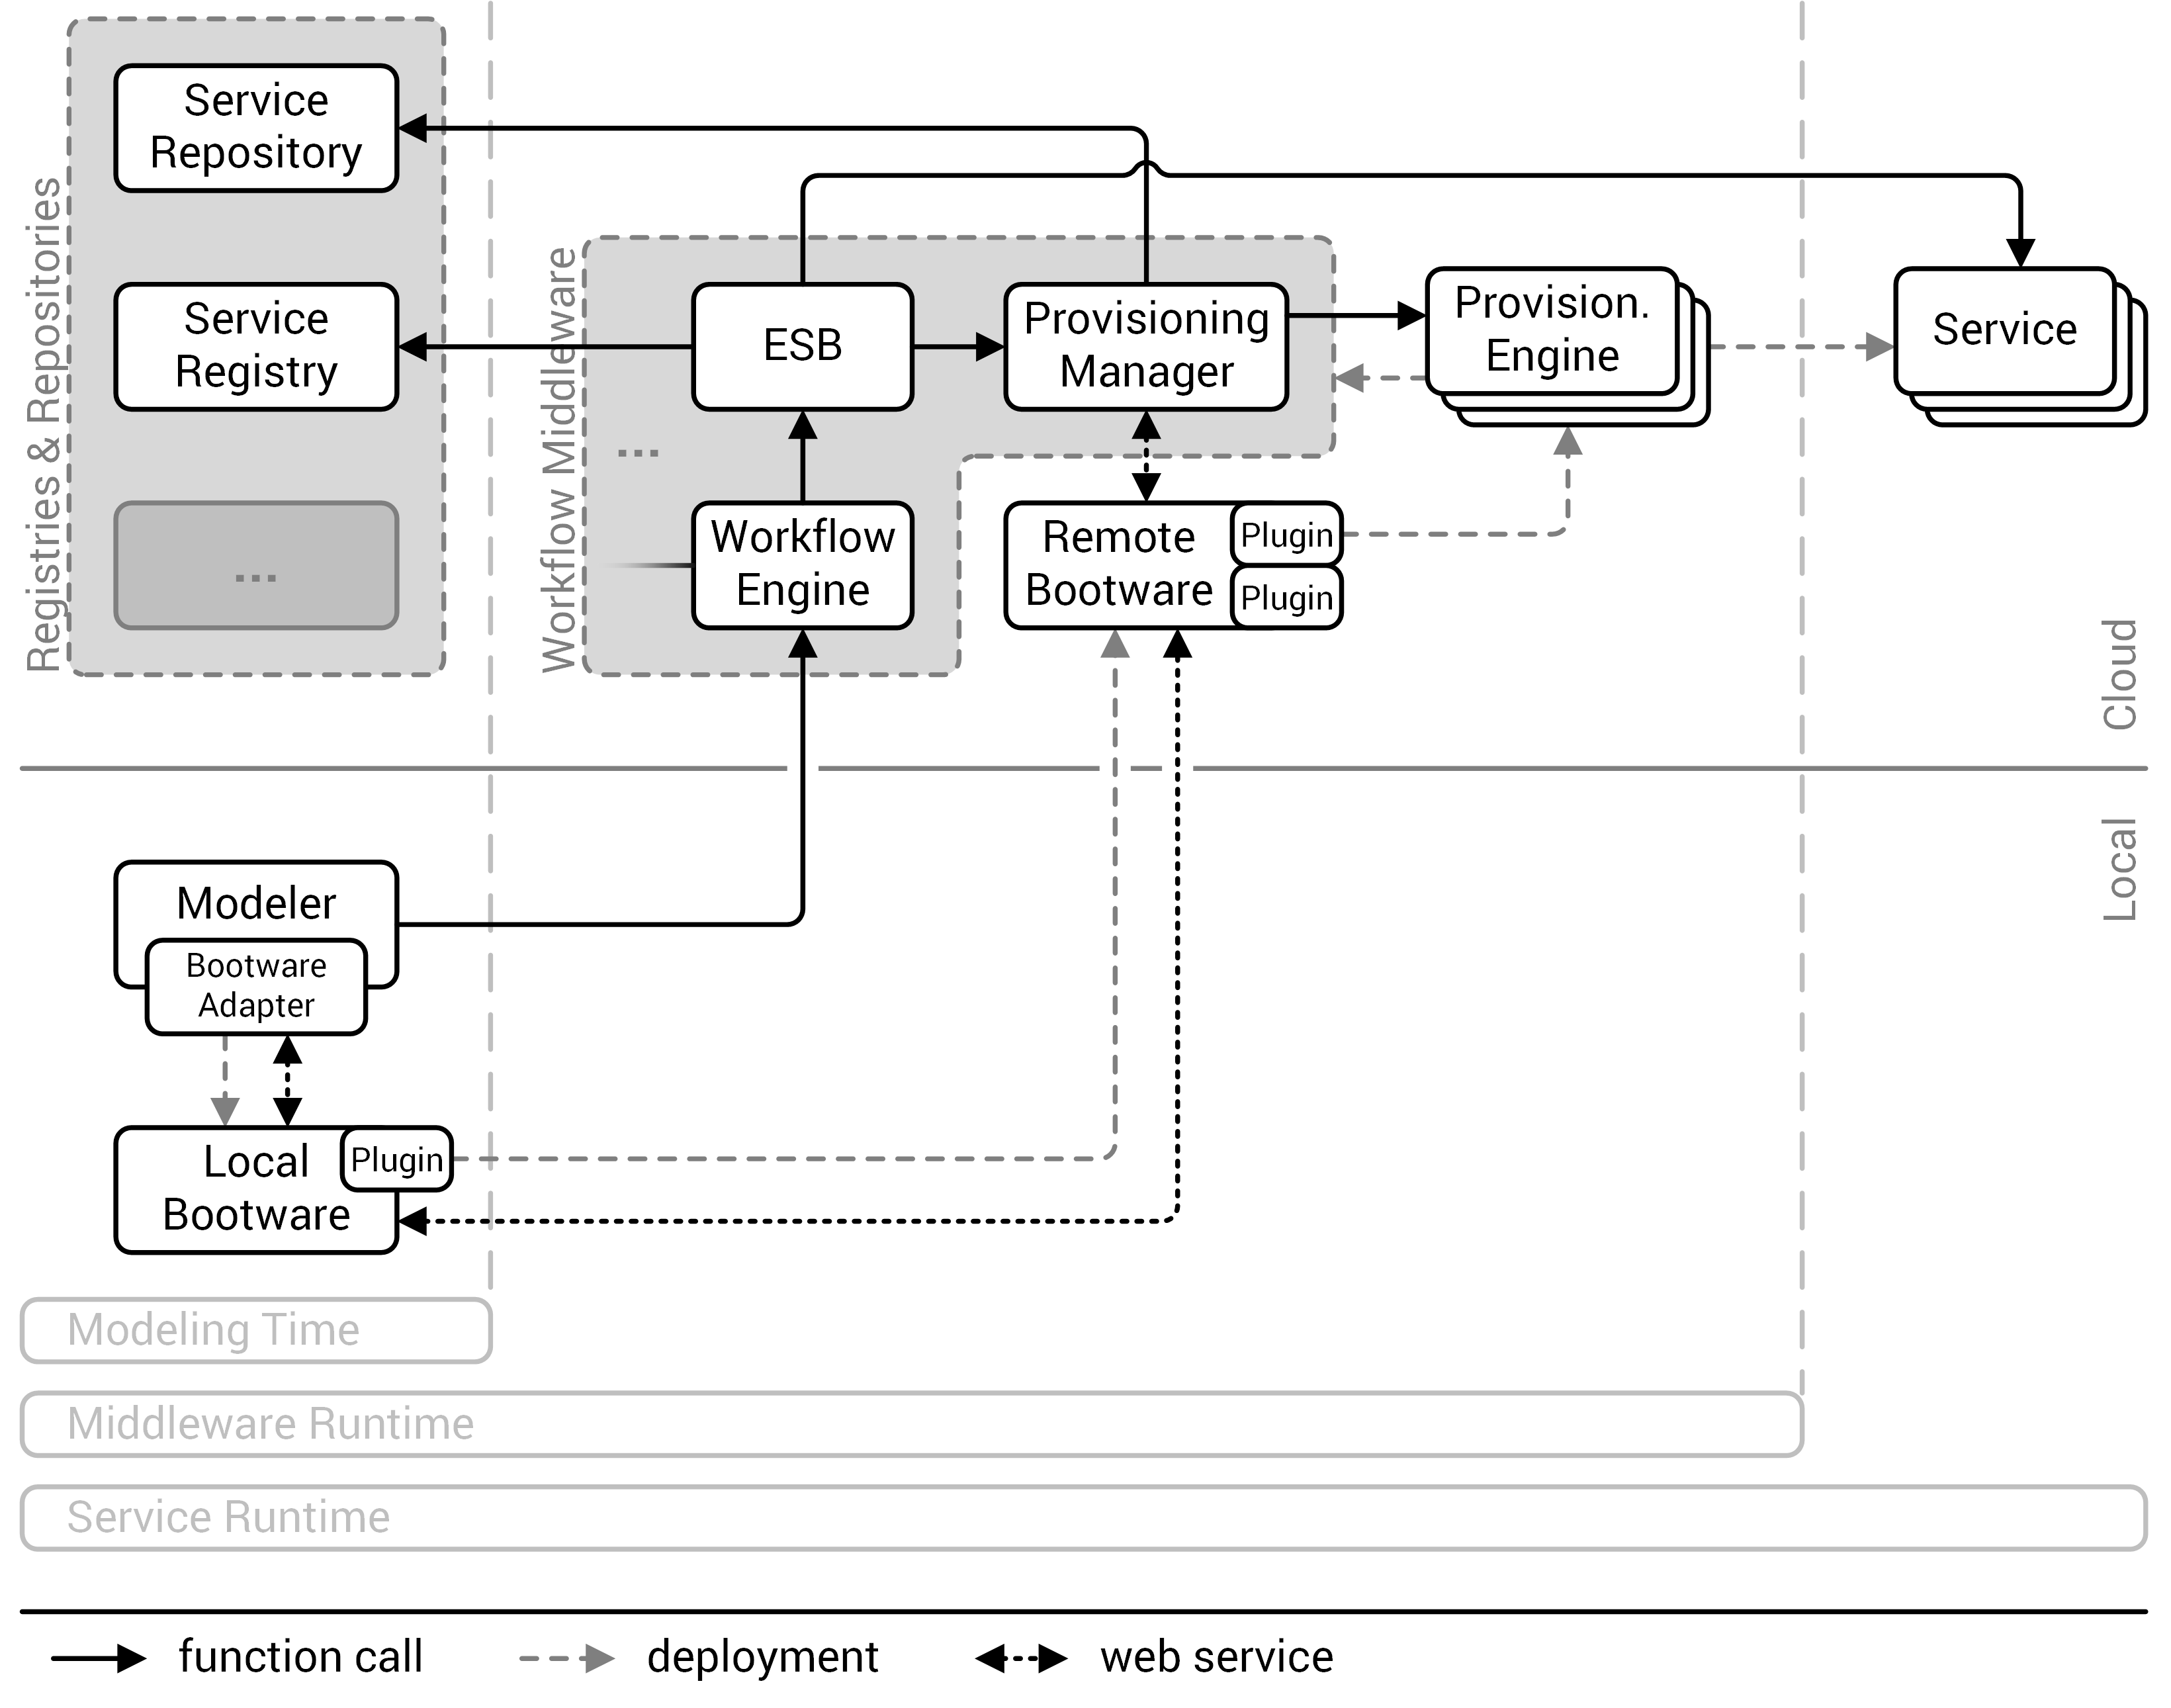
\includegraphics[resolution=600]{design/assets/plugins}
	\caption{Simplified overview of the 2-tier architecture with plugins}
	\label{image:plugins}
\end{figure}

To remedy this situation we introduce a central plugin repository, as shown in \autoref{image:plugin_repository}.
This repository holds all plugins of both components so it eliminates duplicate plugins.
If plugins are added or modified it has only to be done in one place.
Plugin synchronization can happen automatically when the bootware components start, so that the user is no longer involved in plugin management.
The repository also enables easy plugin sharing, which was cumbersome earlier.
While a central plugin repository is a sensible addition to the proposed bootware architecture, its design and implementation are out of scope of this thesis.
This work is left for the future and the plugin repository will not be mentioned in any other figures apart from \autoref{image:plugin_repository}.

\begin{figure}[!htbp]
	\centering
	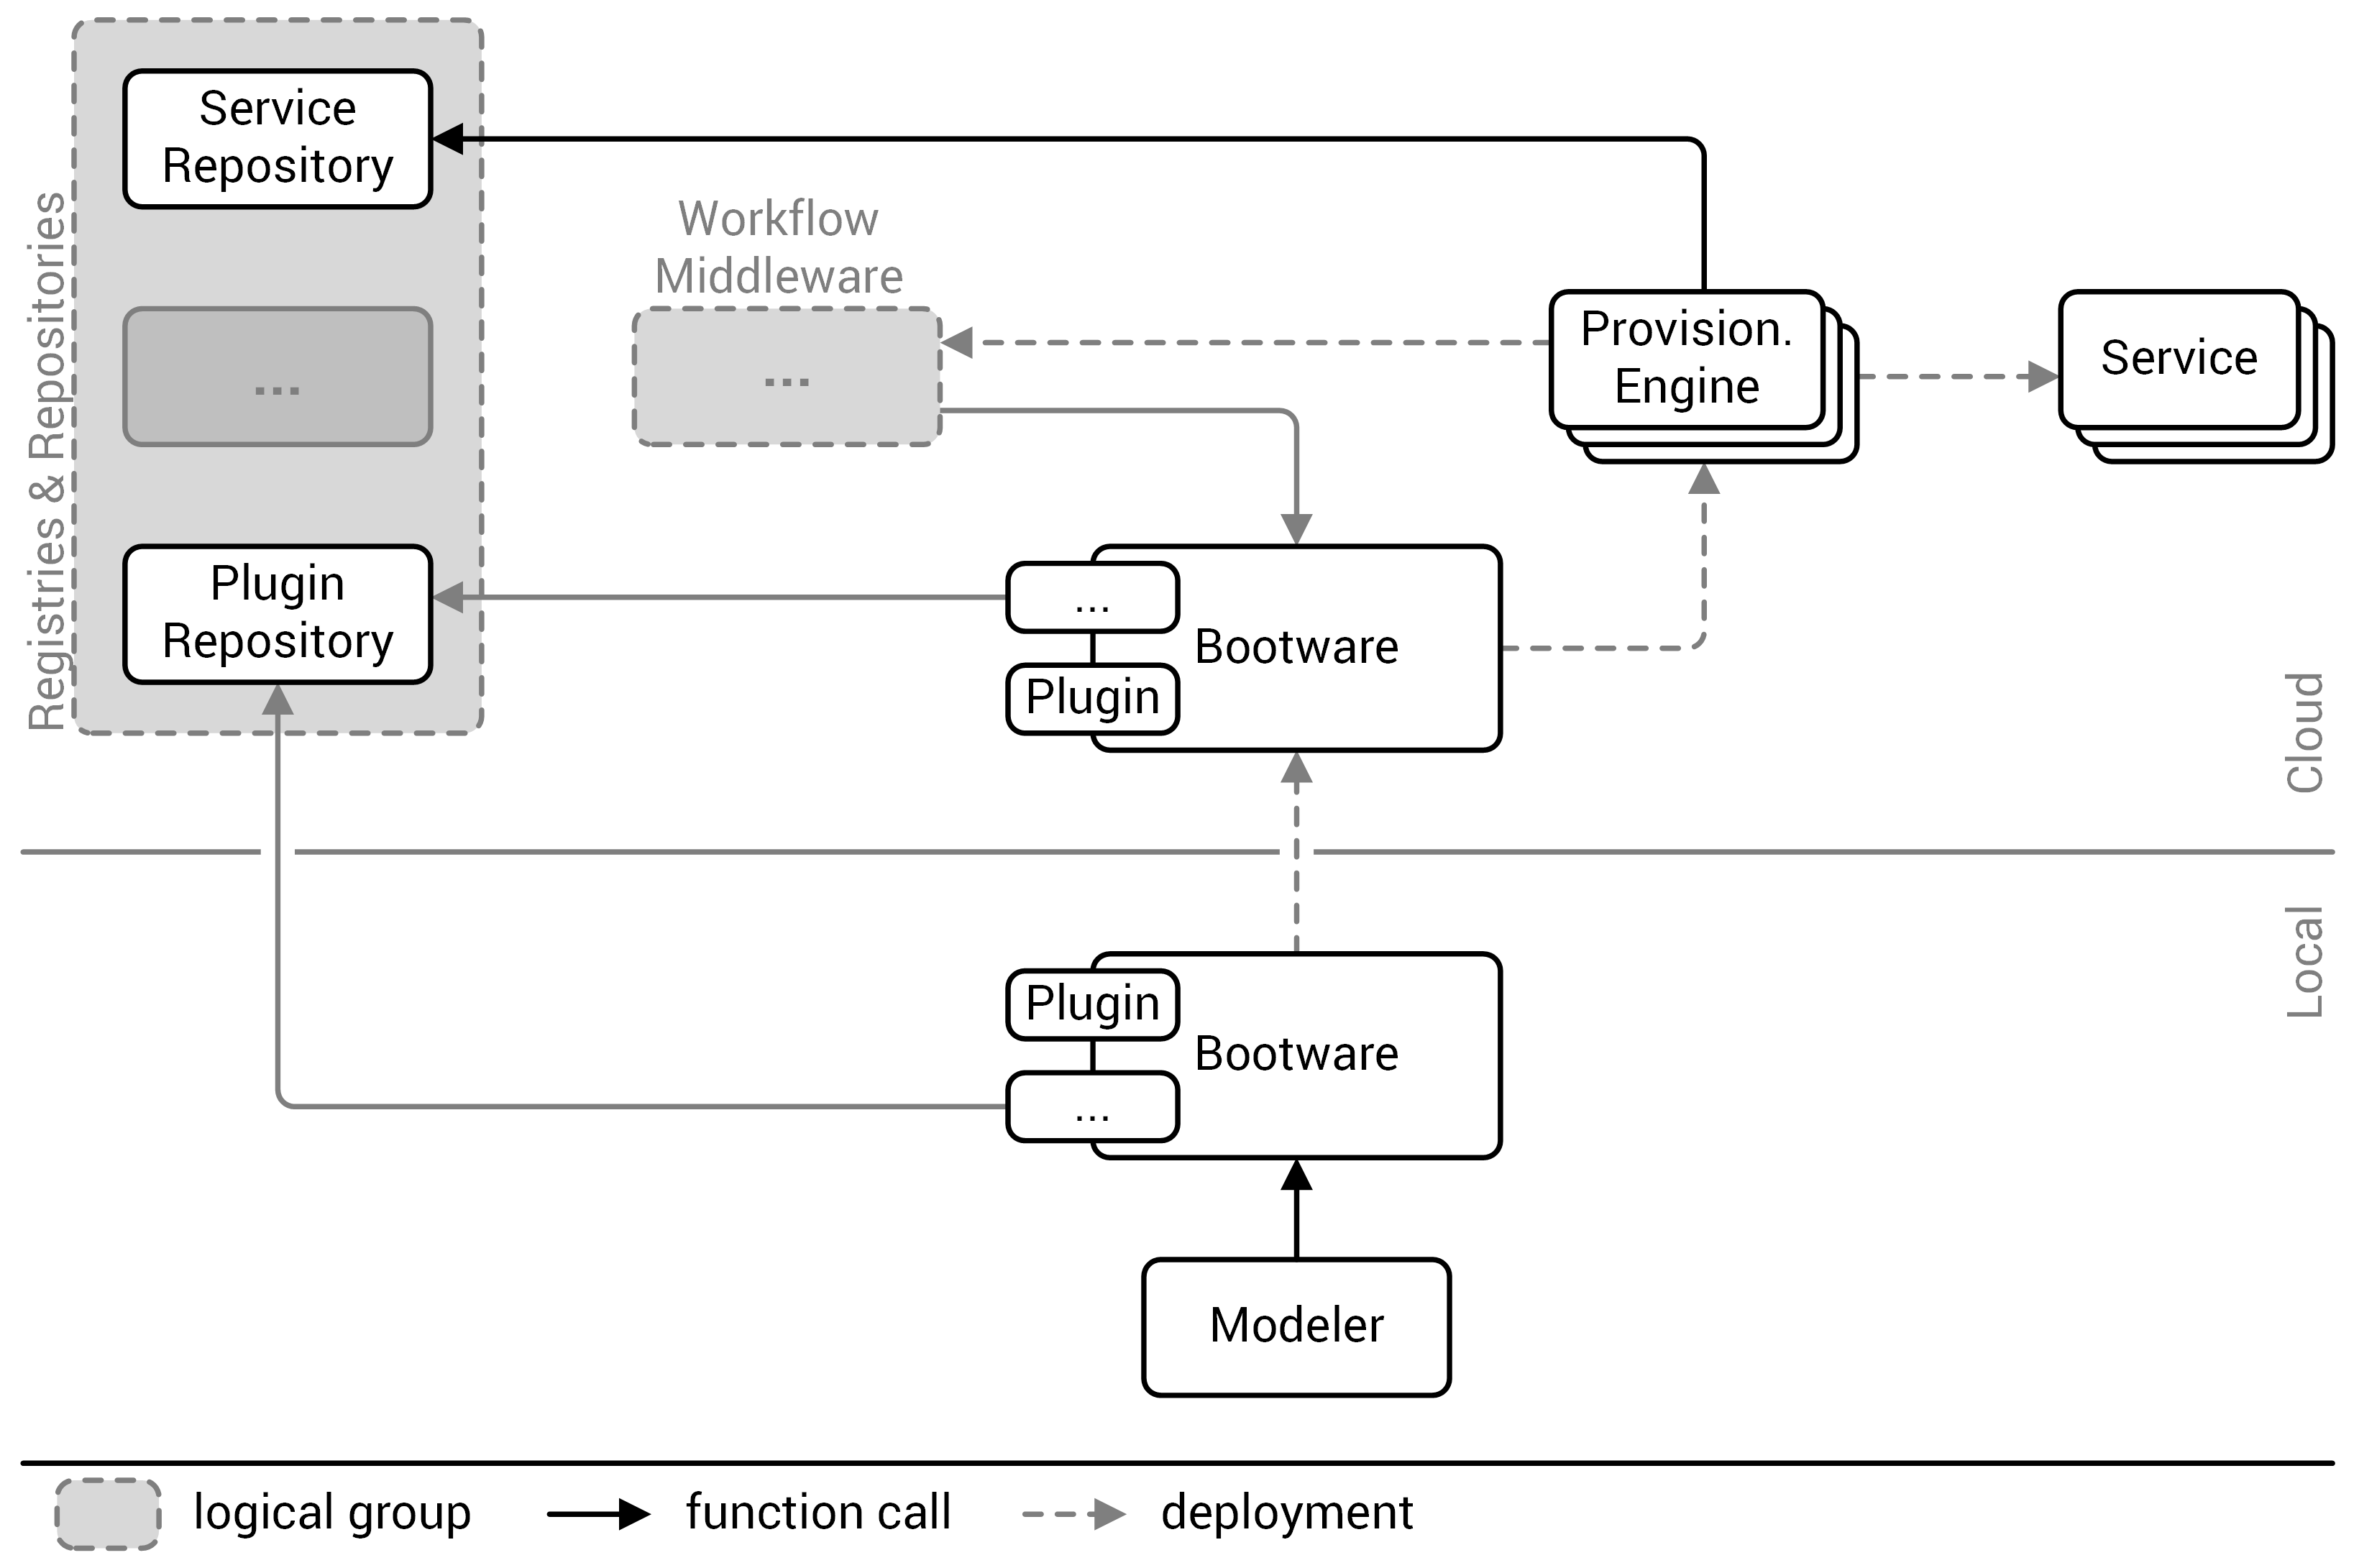
\includegraphics[resolution=600]{design/assets/plugin_repository}
	\caption{Simplified overview of the 2-tier architecture with a plugin repository}
	\label{image:plugin_repository}
\end{figure}
